%% The first command in your LaTeX source must be the \documentclass command.
\documentclass[acmtog]{acmart}
\usepackage[english,ngerman]{babel}
\usepackage[utf8]{inputenc} 

%% \BibTeX command to typeset BibTeX logo in the docs
\AtBeginDocument{%
  \providecommand\BibTeX{{%
    \normalfont B\kern-0.5em{\scshape i\kern-0.25em b}\kern-0.8em\TeX}}}
    
\copyrightyear{2024}
\acmYear{2024}
\citestyle{acmauthoryear}

\usepackage[figurename=Fig.]{caption}
\usepackage{csquotes}
\setcopyright{none}
\makeatletter
\renewcommand{\fnum@figure}{Abb. \thefigure}
\makeatother
\addto\captionsngerman{\renewcommand{\figurename}{Abb.}}
\settopmatter{printacmref=false} % Removes citation information below abstract
\renewcommand\footnotetextcopyrightpermission[1]{} % removes footnote with conference information in first column

\usepackage{minted}

%%
%% end of the preamble, start of the body of the document source.
\begin{document}

%%
%% The "title" command has an optional parameter,
%% allowing the author to define a "short title" to be used in page headers.
\title{Enterprise Architektur-Muster}

%%
%% The "author" command and its associated commands are used to define
%% the authors and their affiliations.
%% Of note is the shared affiliation of the first two authors, and the
%% "authornote" and "authornotemark" commands
%% used to denote shared contribution to the research.
\author{Julian Bruder}
\authornote{Alle Studierenden trugen zu gleichen Teilen zu dieser Arbeit bei.}
\author{Abdellah Filali}
\authornotemark[1]
\author{Luca Franke}
\authornotemark[1]
\affiliation{%
  \institution{Hochschule für Technik, Wirtschaft und Kultur Leipzig (HTWK Leipzig)}
  \streetaddress{Karl-Liebknecht-Str. 132}
  \city{Leipzig}
  \country{Deutschland}
  \postcode{04277}
}
%%
%% By default, the full list of authors will be used in the page
%% headers. Often, this list is too long, and will overlap
%% other information printed in the page headers. This command allows
%% the author to define a more concise list
%% of authors' names for this purpose.
\renewcommand{\shortauthors}{Bruder, Filali, Franke}

%%
%% The abstract is a short summary of the work to be presented in the
%% article.
\begin{abstract}
Blah abstrakt\ldots
\end{abstract}

\maketitle

\section{Einleitung}
% (Beschreibung von Kontext, Problemen, Anforderungen und Zielen)
Mit E-Commerce-Beispiel motivieren

\section{Grundlagen von Enterprise-Architekturen}
Verteilte Systeme \ldots

Architekturen \ldots

Komponenten \ldots

\ldots


\section{Klassische Enterprise-Architekturen}
Blah \ldots

\section{Moderne Enterprise-Architekturen}

\subsection{Microservices Architecture}\label{subsec:microservices}
Die Microservices Architecture zeichnet sich grundlegend durch die Unterteilung der Anwendung in einzelne Service Komponenten aus.
Jede Service Komponente kann vom Umfang und Granularität variieren und enthält bestenfalls eine einzige isolierte Funktionalität
oder einen unabhängigen, größeren Teil der Business Logik.
Diese Service Komponenten bestehen aus einen oder mehreren Modulen, die die Funktionalität des Services implementieren.

Wie in Abbildung~\ref{fig:microservices} dargestellt, werden alle von Clients ausgehenden API-Anfragen zunächst von einem API-Gateway entgegengenommen.
Dieser kommuniziert dann wiederrum über REST-Anfragen mit den Service-Komponenten, die dann die Anfrage verarbeiten und ein Resultat an das Gateway zurückgeben~\cite[30]{architecturePatterns}.

\begin{figure}[!h]
  \centering
  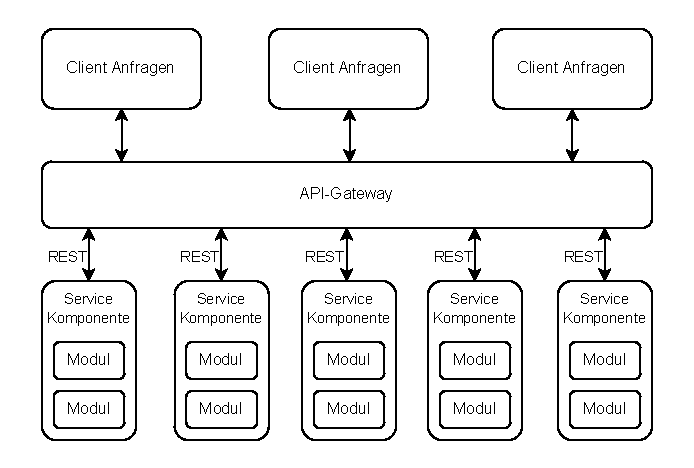
\includegraphics[width=\linewidth]{images/microservices/microservices}
  \caption{Aufbau einer Microservices Architecture}
  \label{fig:microservices}
\end{figure}

Ein maßgebendes Merkmal dieser Architektur-Pattern ist die Entkopplung der einzelnen Services voneinander.
Dies wird dadurch erreicht, dass alle Services nur über ihre definierten Schnittstellen, miteinander kommunizieren können.
Die hohe Entkopplung der Komponenten ermöglicht es, Services unabhängig voneinander zu entwickeln, zu testen und zu deployen.
Pipeline- und Deploymentprozesse finden also isoliert voneinander statt, was die Auslieferung der Software beschleunigt~\cite[27]{architecturePatterns}.

Die richtige Granularität der Services ist entscheidend, um die Vorteile der Microservices Architecture voll auszuschöpfen und stellt hier die größte Herausforderung im Design der Architektur dar.
Werden die Komponenten zu groß gewählt, so kann es passieren, dass die Vorteile der Microservices Architecture nicht mehr greifen.
Innerhalb der Komponenten entstehen Abhängigkeiten, die das isolierte Entwickeln oder Testen von Features verhindern.
Auf der anderen Seite führt eine zu kleine Granularität dazu, dass die Anzahl der Services zu groß wird und das Orchestrieren dieser einen zu großen Overhead verursacht.
Komplexität und Wartungsaufwand steigen stark an und die Schwächen einer klassischen SOA-Architektur treten wieder auf~\cite[32]{architecturePatterns}.

Sollte Kommunikation zwischen den Services notwendig sein, so kann diese über eine geteilte Datenbank stattfinden.
Dadurch werden ungewollte Abhängigkeiten zwischen Services vermieden und die Kopplung der Komponenten verringert.
Dabei ist jedoch darauf zu achten, dass die Datenbank nicht zu einer zentralen Abhängigkeit wird, die die Vorteile der Microservices Architecture wieder zunichte macht~\cite[33]{architecturePatterns}.

%% Hier Beispiel E-Commerce Anwendung

Die Microservices Architektur löst viele der Probleme, die in klassischen monolithischen oder SOA-Architekturen auftreten.
Durch die Aufteilung der Anwendung in kleinere, separat deployte Services, entstehen inhärent robustere und besser skalierbare Systeme.
Da Änderungen oft nur einzelne Service Komponenten betreffen, muss nicht das ganze System neu deployt werden.
Es reicht stattdessen, nur den betroffenen Service zu aktualisieren, was die Ausfallzeiten minimiert und die Wartbarkeit der Software erhöht.
Vor allem in agilen Umgebungen, in denen viele Iterationen und schnelle Auslieferungen notwendig sind, ist die Microservices Architektur daher besonders geeignet~\cite[33]{architecturePatterns}.

Auch können Services in Produktiven-Umgebungen ohne Ausfallzeiten ausgetauscht werden.
Solange, wie der neue Service deployt wird, leitet das API-Gateway Anfragen an den alten Service weiter.
Erst wenn der neue Service bereit ist, werden Anfragen an diesen weitergeleitet und der alte Service kann abgeschaltet werden.

Microservices sind außerdem sehr gut testbar.
Tests können durch die strikte Trennung der Funktionalitäten isoliert auf einzelne Services angewendet werden, ohne dass andere Services betrachtet werden müssen.
Auch Regressionstests nehmen dadurch weniger Zeit in Anspruch.
Kleine Änderungen haben nicht zur Folge, dass die gesamte Anwendung neu getestet werden muss.

Time-to-market bei Microservice Architekturen ist in der Regel kürzer, da deployments schnell sind und parallel an verschiedenen Services gearbeitet werden kann.
Es gibt keine zentrale Abhängigkeit, die sich schwerwiegend auf die Entwicklung einzelner Komponenten auswirken kann.

Der größte Nachteil der sich hier ergibt, ist die vergleichsweise niedrige Performance aufgrund der verteilten Natur des Systems.
Die Kommunikation zwischen Services findet meist über das Netzwerk statt, was zu erhöhten Latenzen führen kann\cite[34]{architecturePatterns}.


\subsection{Microkernel Architecture}\label{subsec:microkernel-architecture}
Die Microkernel Architecture ist ein Architekturmuster, was sich durch Erweiterbarkeit, Flexibilität und vor allem Isolation der Funktionalitäten auszeichnet.
Wie in Abbildung~\ref{fig:microkernel} dargestellt, enthält ein Microkernel zwei wesentliche Komponenten: Den Kern der Anwendung,der die wichtigsten grundlegenden Funktionalitäten bereitstellt und Module oder auch Plugins,
die diesen Kern um Features erweitern~\cite[21-22]{architecturePatterns}.

\begin{figure}[!h]
  \centering
  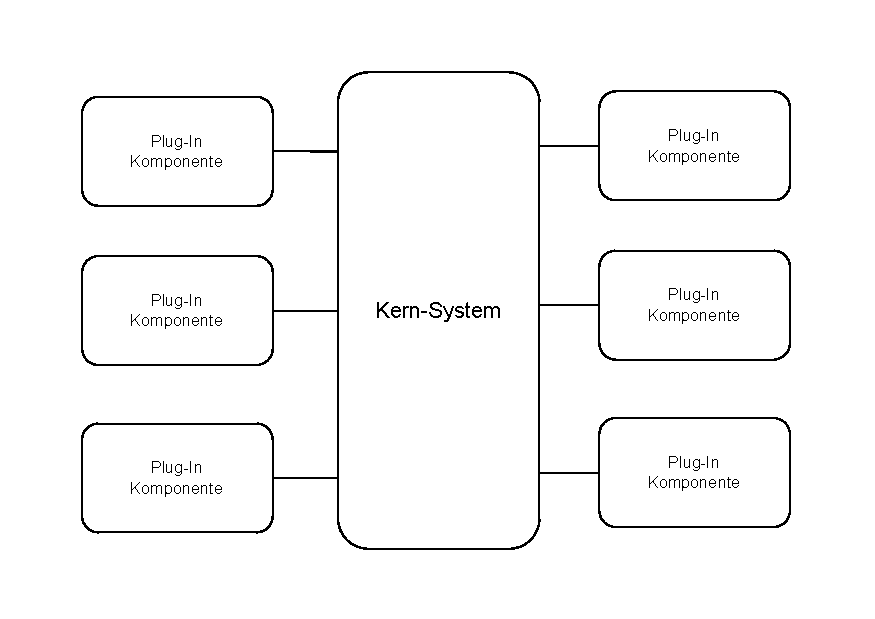
\includegraphics[width=\linewidth]{images/microkernel/microkernel}
  \caption{Aufbau einer Microkernel Architecture}
  \label{fig:microkernel}
\end{figure}

Der Kern der Anwendung implementiert dabei meist nur die minimalste Funktionalität, um die Anwendung oder das System lauffähig zu machen.
Alle weiteren Funktionalitäten werden in Modulen implementiert, die auf den Kern aufbauen.
Module sind meist unabhängig voneinander aufgebaut, es kann jedoch auch vorkommen, dass manche Module von anderen abhängig sind.
Best practice für die Entwicklung von Microkernel Architekturen ist es, die Kommunikation zwischen einzelnen Modulen so gering wie möglich zu halten, um Probleme durch Abhängigkeiten zu vermeiden.
Dadurch sind Module untereinander lose gekoppelt und können unabhängig voneinander entwickelt, getestet und deployed werden~\cite[22]{architecturePatterns}.

Die Plugins können über verschiedene Wege mit dem Kern verbunden werden.
Eine genaue Spezifikation zum Verbinden der Plugins mit dem Kern gibt es aber laut Architekturschema nicht, diese Entscheidung ist dem Entwickler überlassen und entsprechend der Anforderungen und Anwendungsumgebung zu treffen.
Unabhängig von der Art der Verbindung definiert der Kern die Schnittstellen, um Plugins anzubinden.
Diese Verbindung könnte dann beispielsweise über Web-Services, Messaging oder am einfachsten über direkte Objekt-Instanziierung innerhalb der gleichen Anwendung stattfinden~\cite[22-23]{architecturePatterns}.

Zwischen Plugins und Kern werden Verträge definiert, die die Kommunikation zwischen den beiden Komponenten regeln.
Diese Verträge können in Form von Interfaces, Klassen oder auch Datenstrukturen definiert werden.
Alle Plugins, müssen sich zwingend an die definierten Verträge halten, um mit dem Kern kommunizieren zu können.
Alternativ können auch Adapter verwendet werden, um bestehende Plugins an den Kern und die Verträge anzupassen, wodurch wiederrum die lose Kopplung der Komponenten verbessert wird.

Durch diesen Aufbau ergibt sich jedoch das Problem, dass der Kern jederzeit über Verfügbarkeit und Erreichbarkeit der Plugins informiert sein muss.
Um dieses Problem zu lösen, kann eine zentrale Plugin-Registry verwendet werden.
Diese Registry enthält alle aktuell verfügbaren Plugins sowie die dazugehörigen relevanten Informationen wie zum Beispiel Name des Service, Verträge, Verbindungsdetails, etc.
Der Kern der Anwendung kann dann zur Laufzeit auf diese Registry zugreifen und Plugins dynamisch laden~\cite[22]{architecturePatterns}.

Microkernel Architekturen können auch in andere Architekturmuster eingebettet werden, falls es nicht möglich sein sollte die gesamte Software in diesem Architekturmuster aufzubauen.
Vor allem Teile von Anwendungen, die stark erweiterbar sein müssen, eignen sich gut für die Verwendung der Microkernel Architektur.

Ein klarer Vorteil dieses Architekturmusters ist die schnelle Reaktionsfähigkeit auf äußere Änderungen, da Anpassungen aufgrund der losen Kopplung größtenteils nur in den isolierten Modulen vorgenommen werden.
Der Kern der Anwendung ist in den meisten Fällen schnell stabil und benötigt selten im Laufe der Entwicklung weitere Angleichungen.
Geänderte Module können je nach Implementierung auch zur Laufzeit geladen oder hinzugefügt werden, was mögliche Downtime von bereits ausgelieferter Software minimiert~\cite[25]{architecturePatterns}.

Ein Beispiel dafür stellt die Entwicklung von Betriebssystem-Kernels dar, die auch namensgebend für dieses Architekturmuster ist.
Deren Kern Komponenten sind in der Regel sehr stabil und implementieren vor allem grundlegende Funktionen wie Speicherverwaltung, Prozessverwaltung und I/O-Operationen.
Weitere low-level Funktionalitäten wie beispielsweise Geräte Treiber oder Dateisysteme werden als Module in den Kernel geladen und können bei Bedarf hinzugefügt oder entfernt werden, was vor allem für die Unterstützung neuer Hardware wichtig ist.

Auch Entwicklungsumgebungen in der Softwareentwicklung nutzen oft Microkernel Architekturen, um die Support für verschiedene Programmiersprachen und Frameworks zu ermöglichen.

Zwar bietet das Beispiel der E-Commerce Anwendung keinen klassischen Anwendungsfall für Microkernel Architekturen, jedoch kann die Verwendung von Microkernel Architekturen in Teilen der Anwendung trotzdem sinnvoll sein.
Sowohl Zahlungs- als auch Versandfunktionalitäten könnten, wie in Abbildung~\ref{fig:ecommerce-microkernel} dargestellt, in Module ausgelagert werden, um die Anwendung durch weitere Dienstleister erweitern zu können.

\begin{figure}[!h]
  \centering
  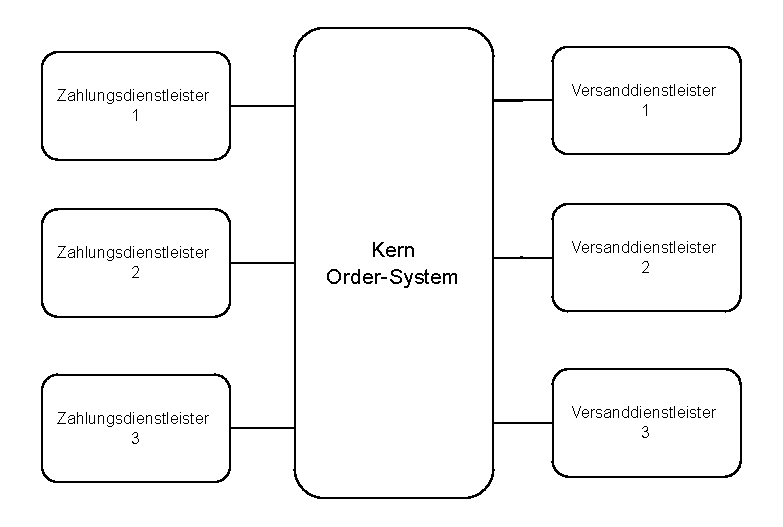
\includegraphics[width=\linewidth]{images/microkernel/ecommerce-microkernel}
  \caption{Aufbau der E-Commerce Anwendung mit Microkernel Architektur}
  \label{fig:ecommerce-microkernel}
\end{figure}

Logik zum Verarbeiten der Zahlungen und Versandinformationen wird dann in den Modulen implementiert, die auf den Kern der Anwendung aufbauen.
Dabei ist jedoch ein Großteil der Business-Logik im Kern der Anwendung enthalten, was nicht dem eigentlichen Gedanken der Microkernel Architektur entspricht.

Abgesehen davon erhöhen Microkernel Architekturen inhärent die Testbarkeit der Software, da Module nur lose Kopplung gekoppelt sind.
Jedes Modul kann unabhängig voneinander getestet werden und fehlende Module durch Stubs ersetzt werden, wodurch sich während der Entwicklung auf einzelne Module isoliert konzentriert werden kann~\cite[26]{architecturePatterns}.
Weiterhin können Verhaltensweisen von anderen Modulen durch Mocks simuliert werden, um Testzustände zu erzeugen und das Verhalten der Anwendung zu verifizieren.
In Agilen Umgebungen, in denen das Testen von Software eine wichtige Rolle spielt, ist die Verwendung von Microkernel Architekturen daher besonders sinnvoll.

Eine Herausforderung bei der Verwendung von Microkernel Architekturen kann jedoch der Entwurf der Kern-Komponente darstellen.
Da alle anderen Module auf den Kern aufbauen, muss dieser sehr sorgfältig und stabil entwickelt werden, um die Funktionalität der gesamten Anwendung zu gewährleisten.
Diese Rolle sollten vor allem erfahrene Entwickler übernehmen, da sich Design-Fehler der Kern-Komponente oder Verträge negativ auf die Entwicklung der Module auswirken können.
Sollte der Kern der Anwendung angepasst werden, so müssen tendenziell auch alle Module überprüft oder aktualisiert werden, was zu erheblich erhöhten Entwicklungszeiten führen kann und zuvor gewonnene Vorteile der Microkernel Architektur zunichte macht.

Aufgrund der initial hohen Komplexität, die mit der Entwicklung des Kerns einhergeht, stellt die Microkernel Architektur nicht die beste Wahl dar, wenn es darum geht schnell eine erste Version der Software auf den Markt zu bekommen.
Die wesentlichen Vorteile, die die Microkernel Architektur bietet, zeigen sich erst im späteren Verlauf der Entwicklung, wenn die Anwendung erweitert werden muss.
Sowohl Iterationen als auch Auslieferungszeiten sind dann sehr kurz, da Module unabhängig voneinander entwickelt werden und die Anwendung schnell an neue Anforderungen angepasst werden kann.
Diese Vorteile können die Architektur in ausgewählten Anwendungsfällen sehr geeignet für agile Entwicklungsumgebungen machen.

\subsection{Event-Driven Architecture}
Die Event-Driven Architecture wählt als Basis einen anderen Ausgangspunkt als die bisherigen Architekturmuster.
Während bei letzteren Komponenten Dienste bereitstellen, welche von anderen Komponenten explizit genutzt werden,
verhalten sich Dienst-bereitstellende Komponenten in der Event-Driven Architecture reaktiv,
werden also implizit von Dienst-konsumierenden Komponenten genutzt \cite{garlanShawImplizit}.
Ein System reagiert somit asynchron auf Zustandsänderungen, also Ereignisse in diesem System \cite{eda}.
Die in dieser Architektur minimalen Einheiten, welche Informationen einer Zustandsänderung kapseln, werden \textit{Events} genannt.
Die Idee der impliziten Behandlung von Ereignissen ist nicht neu und taucht erstmals 1994 im von Garlan und Shaw publizierten Papier
\textit{\enquote{An introduction to Software Architecture}} auf.

Betrachten wir im Folgenden die Basis-Bestandteile der Event-Driven Architecture:
\begin{itemize}
  \item Ereignis (englisch \textit{Event}): Kapselt Information einer Zustandsänderung eines Systems
  \item Produzent (englisch \textit{Producer}): Komponente, die Event erzeugt
  \item Herausgeber (englisch \textit{Publisher}): Komponente, die, von Produzenten erzeugte, Events publiziert
  \item Konsument (englisch \textit{Consumer}): Komponente, die auf publizierte Events reagiert
  \item Vermittler (englisch \textit{Mediator}): Komponente zwischen Produzenten und Konsumenten - filtert Events und verteilt diese auf Konsumenten
  \item Event-Bus: Oft auch \textit{Event-Broker} genannt - bietet die Infrastruktur für die Gesamtheit der Vermittler
\end{itemize}
Abstrakt kann ein Event als Vertrag zwischen Produzenten und Konsumenten am Event-Bus betrachtet werden.
Der Konsument nutzt die Spezifikation des Events am Bus, der Produzent implementiert jene Spezifikation.
Abbildung \ref{fig:eda} stellt diesen Vertrag dar.

\begin{figure}[!h]
  \centering
  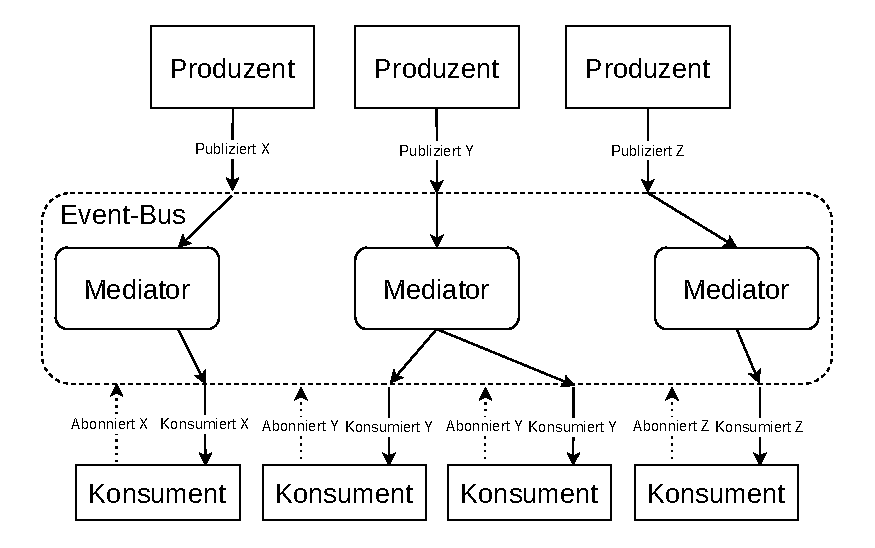
\includegraphics[width=\linewidth]{images/eda/eda.drawio}
  \caption{Vertrag zwischen Produzenten und Konsumenten am Event-Bus}
  \label{fig:eda}
\end{figure}

Durch den Vertrag weisen die Events am Event-Bus starke Kohäsion und somit lose Kopplung auf.
Diese lose Kopplung minimiert nicht nur kaskadierende Fehler, sondern ermöglicht agilen Entwickler-Teams durch klar abgegrenzte Features einfach definierbare Iterationen
- eine Menge von Events, deren Erzeugung und Konsumierung.

Weiter sind Events oft nah an dem, was Ereignisse in realen Prozessen sind, also domain-driven.
Gebündelt ermöglichen obige Punkte die kontinuierliche Auslieferung von Software in kurzen Intervallen.

Außerdem garantiert die asynchrone Behandlung von Ereignissen zusammen mit der loosen Kopplung maximale Skalierung.
Daher sind Event-Driven Architekturen besonders für datenintensive Echtzeit-Anwendungen wie IoT (Internet of Things) und Analytics geeignet \cite{iotEda}.

Betrachten wir erneut das E-Commerce-Beispiel aus der Einleitung.
Dafür definieren wir drei Arten von Events:
\begin{itemize}
  \item \texttt{OrderCreated}: Ein Event, das genau dann erzeugt wird, wenn eine neue Bestellung aufgegeben wird
  \item \texttt{PaymentProcessed}: Ein Event, das genau dann erzeugt wird, wenn der Bezahlvorgang abgeschlossen wird
  \item \texttt{ShipmentInitiated}: Ein Event, das genau dann erzeugt wird, wenn die Bestellung versandt wird
\end{itemize}

Weiter teilen wir die Funktionalität ähnlich wie bei der Microservice-Architektur in die drei verschiedenen Dienste \texttt{OrderService}, \texttt{PaymentService} und \texttt{ShipmentService} auf.

\begin{figure}[!h]
  \centering
  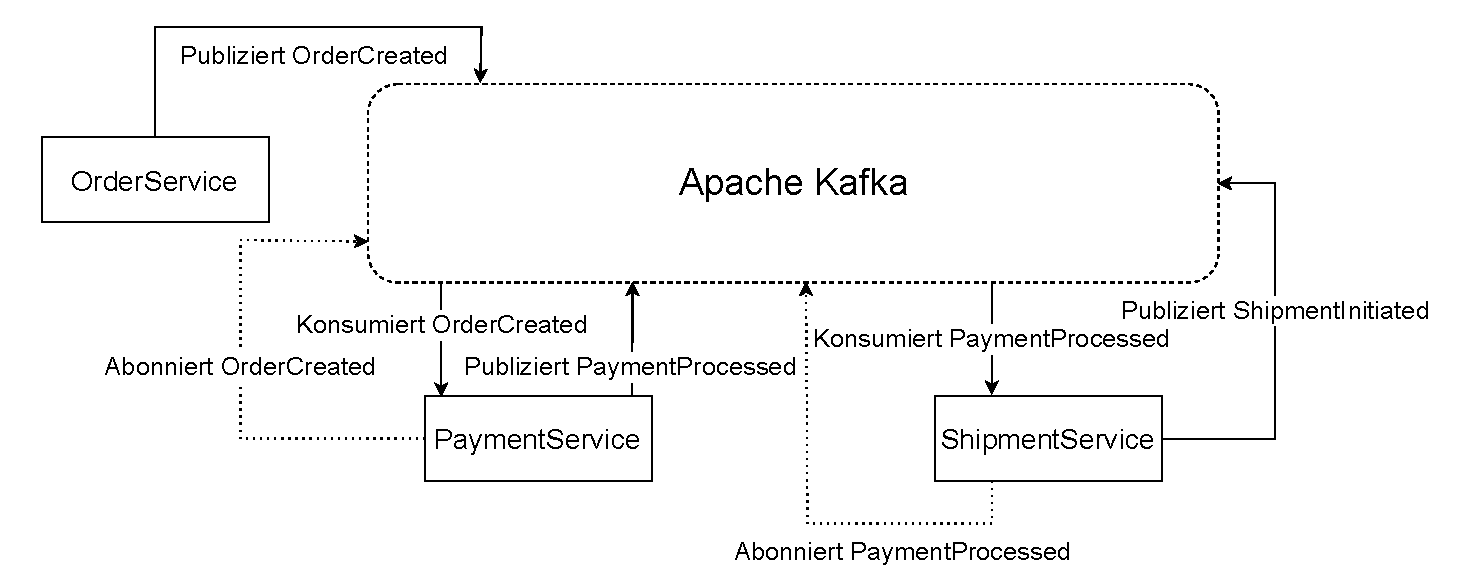
\includegraphics[width=\linewidth]{images/eda/eda-ecommerce.drawio}
  \caption{E-Commerce-Beispiel mit Event-Driven Architecture}
  \label{fig:edaecommerce}
\end{figure}
Wie Abbildung \ref{fig:edaecommerce} zeigt, sind alle drei Dienste Produzenten und Publisher, erzeugen also Events und veröffentlichen diese.
Die Dienste \texttt{PaymentService} und \texttt{ShipmentService} sind zudem Konsumenten,
sodass ersterer auf Events des Typs \texttt{OrderCreated} und zweiterer auf Events des Typs \texttt{ShipmentInitiated} reagiert.
Eine beispielhafte Implementierung des \texttt{PaymentService} mit Apache Kafka als Event-Broker ist im Anhang \ref{app:code:eda:paymentservice} zu finden.
Die vollständige Implementierung des E-Commerce-Beispiels ist bei GitHub \footnote{https://github.com/Beleg-6-EAP/demo-eda-ecommerce} zu finden.

Das Beispiel zeigt, dass die Event-Driven Architektur mit weiteren agilen Strukturen wie Microservices kombiniert werden kann, was die Agilität der Architektur weiter erhöht.
Die damit einhergehende Komplexität stellt teilweise hohe Anforderungen an die Entwickler.
Aufgrund der Asynchronität der Behandlung von Ereignissen ist die Testung des Systems meist schwer und die Fehlerbehandlung essentiell.
Mögliche Problemquellen schließen dabei unter anderem Event-Verlust, erhöhte Latenz und Inkonsistenz ein.
Die hohen Anforderungen an die Entwickler verlangen viel Vertrauen in jene, einer der zentralen Punkte des agilen Manifests \cite{agileManifesto}.
Insgesamt weist die Event-Driven Architecture also eine sehr hohe Agilität auf und ist damit besonders für moderne Software und ihre stetig wechselnden Anforderungen geeignet.

\section{Fallstudien und Praxisbeispiele}
Blah \ldots

\section{Diskussion}

\section{Zusammenfassung und Ausblick}
%(Überblick über die gesamte Arbeit, Rückführung auf Aussagen aus Kapitel 1 durchführen, offene Punkte als neue Forschungsfragen definieren)






\bibliographystyle{ACM-Reference-Format}
\bibliography{main}

\appendix

\section{Code-Beispiele}

\subsection{Event-Driven-Architecture}
\label{app:code:eda:paymentservice}
\begin{listing}[H]
  \tiny
  \inputminted[linenos=true]{java}{code/eda/PaymentService.java}
  \caption{Service-Implementierung des \texttt{PaymentService} in Java Spring Boot 3.4.1 mit Apache Kafka als Event-Broker}
  \label{listing:semigroup}
\end{listing}

\section{Übungsaufgaben}
\subsection{Übungsaufgabe 1 }
Blah \ldots

\end{document}
\endinput
